\section{Hydraulics of sewer line}\label{se:hydraulics_of_sewer_line}

Methods to model hydraulics of gravity and pressurized sewer line is explained respectively in the following. 

Modeling fluids is almost always done by considering it as a control volume, as it is rarely efficient or possible to consider the individual fluid particles.
Henceforth the control volume will be denoted by the letter $\Omega$ which will correspond to some amount of fluid in a length of sewer line.

The open channel flow in gravity sewer lines can be described by the Saint-Venant equations which gives an expression for conservation of mass and momentum.
Some assumptions is made when utilizing the Saint-Venant equations:
\begin{table}[H]
\begin{enumerate}
\item The flow in the channel is one dimensional and as such any curvature of the sewer line is neglected.
\item Fluid in the sewer line is incompressible i.e. the pressure is assumed hydrostatic.
\item The only forces considered is friction and gravity.
\item 




\item The flow in the sewer is one-dimensional, meaning that the water height and velocity is uniform in the cross-section and only changes horizontally.
\item The curvature of the sewer line is sufficiently small such that it can be considered a straight line. 
\item Vertical accelerations is neglected and the fluid is incompressible such that the pressure can be assumed hydrostatic.
\item The slope and the variation in width of the sewer line is small.
\item The effect of scour and accumulation of solids are assumed to be negligible. 
\end{enumerate}
\label{tab:saintbernard_assumptions}
\end{table}


\begin{figure}[H]
\centering
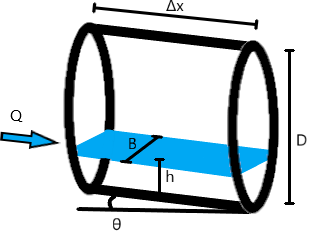
\includegraphics[width=0.45\textwidth]{report/modeling/pictures/kloakroer.png}
\caption{Sewer pipe \fxnote{Ny tegning}}
\label{fig:kloakroer}
\end{figure}



\begin{equation}	
\frac{\partial A(x,t)}{\partial t} + \frac{\partial Q(x,t)}{\partial x}=q(x,t)
\label{saintbernard_mass}
\end{equation}

where:
	Q = volumetric flow rate ($\frac{M^3}{s}$)
	A = cross section of the water volume $m^2$
	q = lateral inflow of water $\frac{m^2}{s}$



\begin{equation}
	\frac{\partial Q(x,t)}{\partial t} + \frac{\partial}{\partial x} \frac{Q^2(x,t)}{A(x,t)}+ g A(x,t) (\frac{\partial Y(x,t)}{\partial x} +S_f(x,t)-S_b(x)) = 0
\label{saintbernard_momentum}
\end{equation}

\begin{equation}
	S_f = \frac{Q^2n^2}{A^2R^{4/3}}
\label{Manning_formula}
\end{equation}
\subsection{Preissmann scheme}\label{subse:preissmann_scheme}



